\chapter{Introduction} % Main chapter title
\label{chap:intro} % Change X to a consecutive number; for referencing this chapter elsewhere, use \ref{ChapterX}

%----------------------------------------------------------------------------------------
%	SECTION 1
%----------------------------------------------------------------------------------------

\section{Background and motivation}
Noise pollution is becoming more and more serious nowadays due to the development of transportation systems (e.g., cars, airplanes, ships, trains), manufacturing plants (e.g., transformer stations), electrical appliances (e.g., vacuum cleaners, refrigerators, air-conditioners), and so on \cite{Hogan1973RelationshipHighwayPlanning}. 
    Exposures to high levels of noise could cause health issues to human beings, such as the hearing loss, cardiovascular diseases, cognitive impairment, and tinnitus \cite{WorldHealthOrganization2011BurdenDiseaseEnvironmental, Munzel2014CardiovascularEffectsEnvironmental}.
    Therefore, it is necessary to control the noise levels.
Noise can be mitigated at three different stages: at the noise source, along the wave propagation path, and at the human ear (receiver). 
Different noise control techniques have been proposed to control noise at different stages.

Passive noise control (PNC) techniques include the installation of enclosures covering noise sources \cite{2000ISO156672000, 2009ISO1154612009}, building sound barriers and insulation walls in highways, around airports, and construction sites \cite{Kurze1974NoiseReductionBarriers, Tong2015FullScaleField}, and wearing earplugs and earmuffs around the human ears \cite{Gerges2012EarmuffComfort}. 
    The size of the devices and/or materials used in PNC techniques (e.g., porous absorbers \cite{Allard2009PropagationSoundPorous, Padhye2016AcousticTextiles} and Helmholtz resonators \cite{Cai2016NoiseControlZone}) depends on the wavelength and is usually sizable at low frequencies, which may limit their applications when there are weight and volume constraints.
    Active noise control (ANC) is a method to mitigate noise at target regions by introducing additional loudspeakers (called \quotes{secondary sources}) \cite{Nelson1992ActiveControlSound, Qiu2019IntroductionVirtualSound}.
It provides an alternative solution to control the low frequency noise.
The theory and physical mechanism of ANC methods have been well established and investigated, and successful applications include the ANC systems in headphones \cite{Ang2017PerformanceActiveNoisecanceling}, headrests in cars \cite{Jung2018EstimationPressureListener, Elliott2018HeadTrackingExtends}, domenstic windows enabling natural ventilation \cite{Lam2019ActiveControlNoise, Lam2020ActiveControlBroadband}, and so on \cite{Lam2021TenQuestionsConcerning}.

Figure~\ref{fig:anc_structure} shows the typical structure of an ANC system.
    In practice, the unwanted noise is time varying, so a controller is required to process the real time audio signals.
    The reference sensors (e.g., microphones or tachometers) are placed near the noise source (called the \quotes{primary source}) to capture the noise signal, which is called the \quotes{reference signal}.
    The error sensors (e.g., microphones or accelerometers) are used to obtain the residual noise level at the error points.
    The reference signals are filtered by control filters in the controller to generate the real time anti-noise signal for secondary sources, resulting in a noise reduction at error points.
    There are various kinds of algorithms to obtain the control filters,
    all of which aim to maximize the noise reduction level at error points.
    The filtered-x least mean square (FxLMS) algorithm is desgined to minimize the sum of the square of sound pressure at all error points \cite{Elliott2000SignalProcessingActive}. 
    It has low computational cost, stable performance, and commonly employed in commercial ANC controllers, so it is adopted in this work.

\begin{figure}[!htb]
    \centering
    % 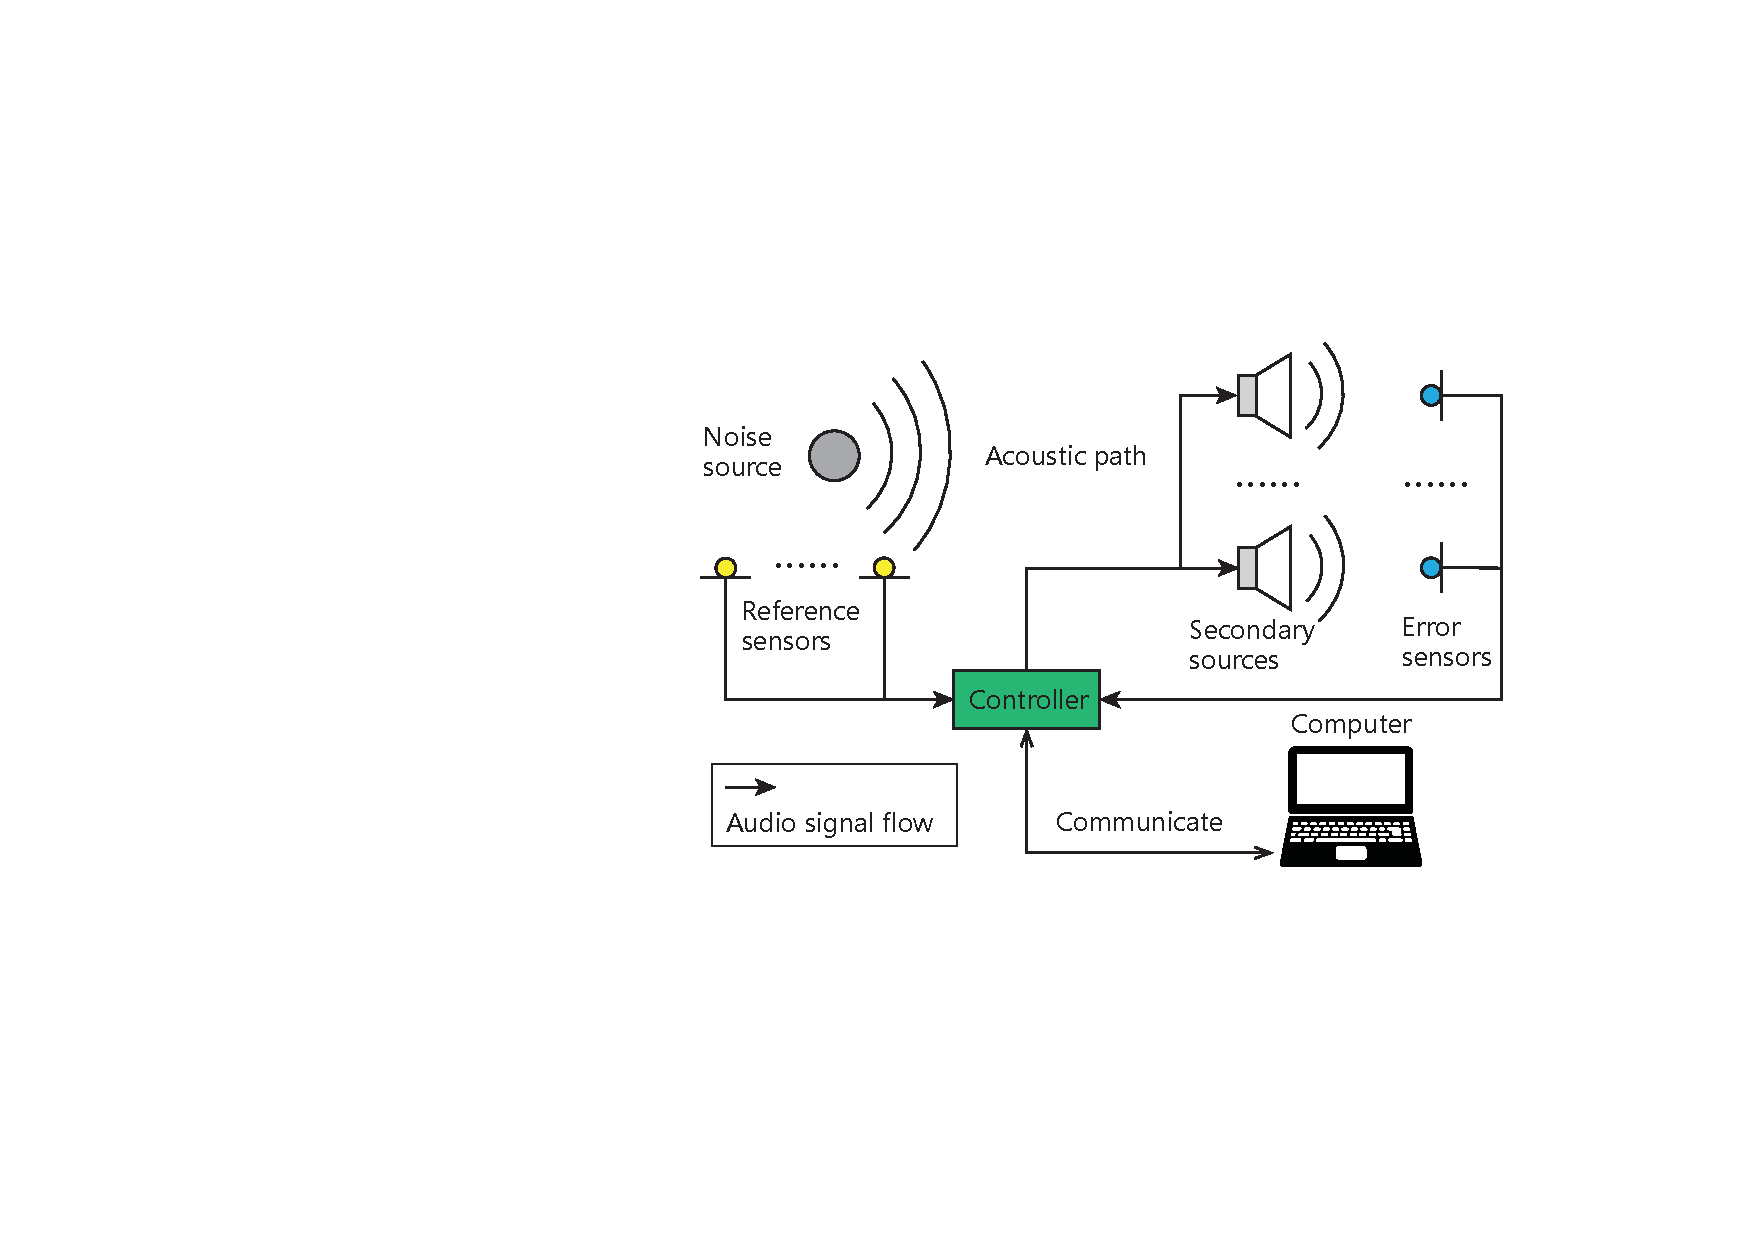
\includegraphics[width = 0.6\textwidth]{fig/ANC_structure/ANC_structure_211117A.pdf}
    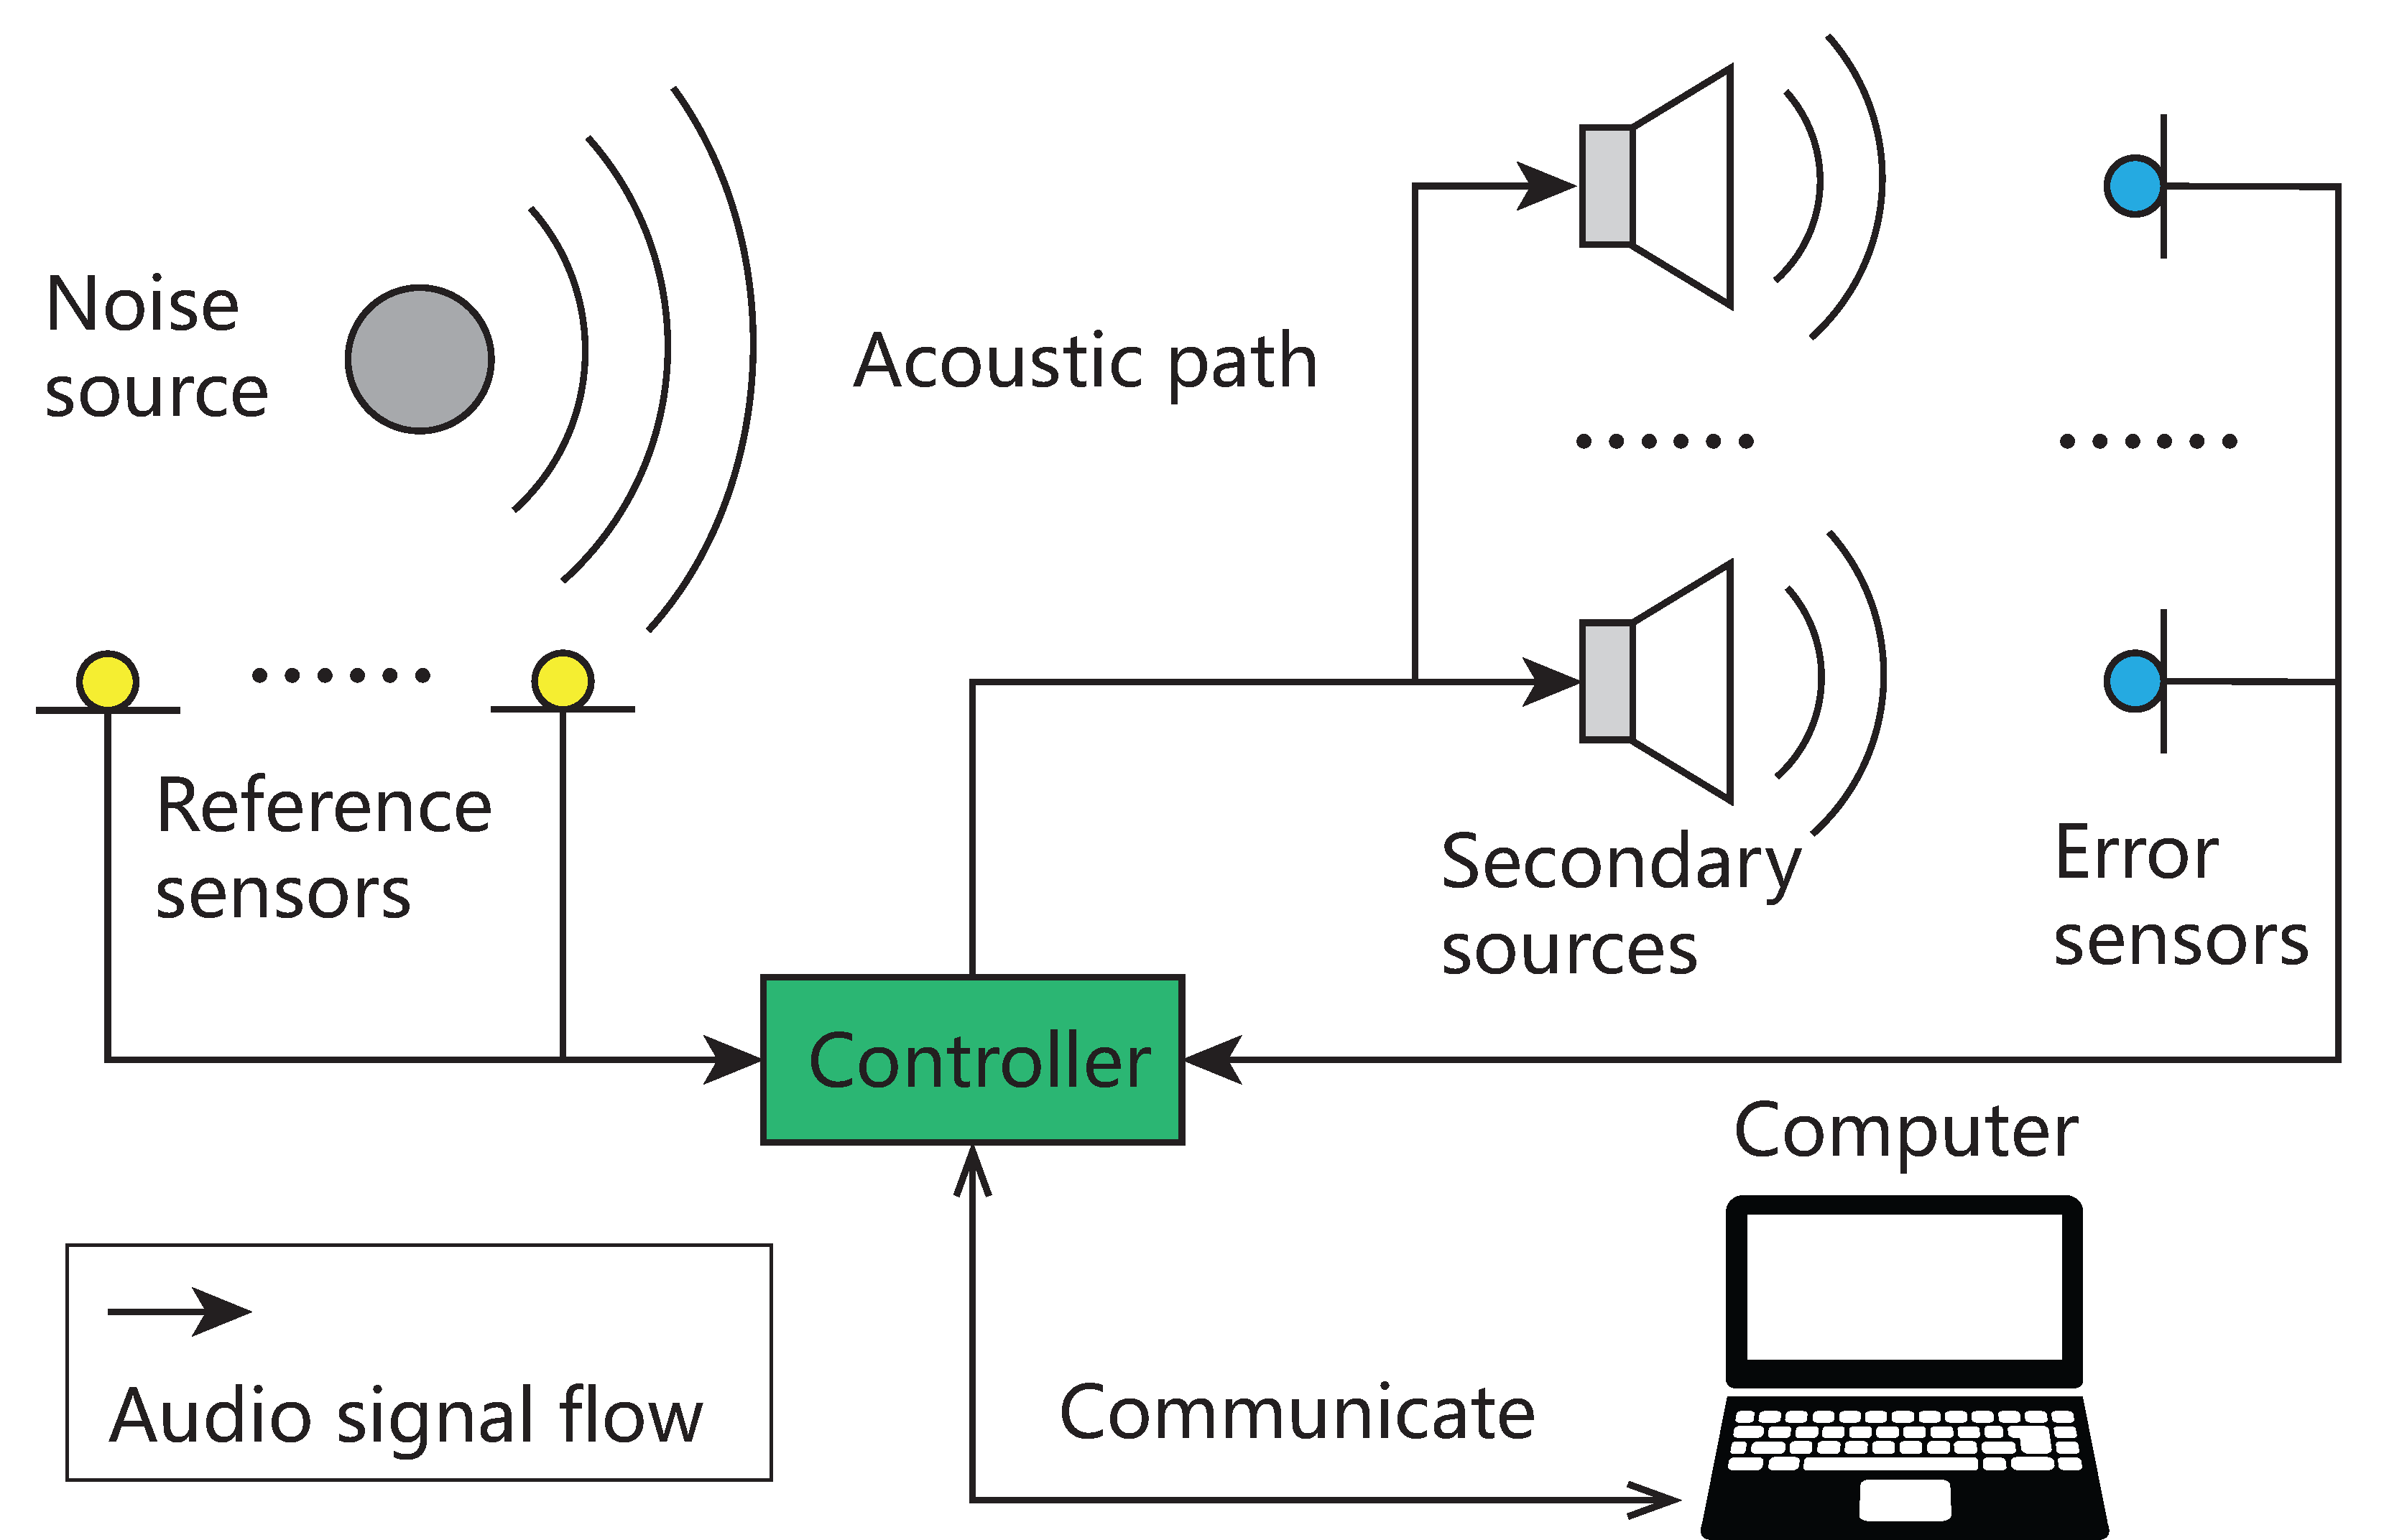
\includegraphics[width = 0.6\textwidth]{fig/ANC_structure/ANC_structure_211117A.png}
    \caption{Structure of an ANC system.}
    \label{fig:anc_structure}
\end{figure}

%% todo: insert a figure to show the examples mentioned above

    There are two strategies of ANC systems, namely global active control and local active control \cite{Nelson1992ActiveControlSound}.
    The global active control aims to reduce the total sound power radiated from the noise and secondary sources \cite{Boodoo2015ReviewEffectReflective}. 
    Although the radiation of the system can be globally mitigated when the distance between secondary and noise sources is small, the noise reduction performance deteriorates significantly when the distance is larger than half of a wavelength \cite{Zhong2019IncreasingPerformanceActive, Zhong2019IncreasingPerformanceActivea, Zhong2020PerformanceActiveNoise}.
    When global control cannot be achieved, local active control can be used to mitigate the noise in a particular region and form a so called \quotes{quiet zone}, which is defined as the region where the noise reduction is larger than 10 dB \cite{Guo1998EffectsReflectiveGround, Elliott2015ModelingLocalActive, Shi2020MultichannelActiveNoise}.
    It is noted that the sound field in other areas is not taken into account in the local active control strategy.
    When the traditional dynamic loudspeakers are used as secondary sources in ANC systems, 
    the noise in some other areas outside the quiet zone can be amplified 
    because traditional dynamic loudspeakers are approximately omnidirectional.
    This phenomenon is referred to as the \quotes{spillover effect} in the literature \cite{Guo1997ActivelyCreatedQuiet, Kidner2006FeasibilityStudyLocalised, Tanaka2010ActiveNoiseControl}.

To illustrate the spillover effect, Fig.~\ref{fig:intro:389fsdp} is presented showing the physical configuration of a single channel ANC system.
When a secondary source (denoted by a cross mark) is used to cancel the noise radiated by a point source (denoted by a circle mark) at an error point (denoted by a square mark), 
the quiet zone is formed around the error point.
The spillover effect can be observed that the sound pressure in some other areas is amplified due to the omnidirectional sound waves generated by the traditional secondary loudspeakers, which is undesirable in real applications.
Moreover, such property increases the instability of the ANC system because the reference signal is contaminated by the secondary source signal received by the reference sensors \cite{Tanaka2010ActiveNoiseControl}. 
As shown in Fig.~\ref{fig:anc_change_dist}, placing the secondary source close to the target point can mitigate the increase of total energy in the other areas \cite{Joseph1994FieldZonesQuiet, David1994NumericalStudiesActively}, 
but it reduces the quiet zone size \cite{Guo1998EffectsReflectiveGround}, 
and also brings extra obstructions to the target point.
    The spillover effect is annoying in applications.
    For example, when a quiet zone is created in the main driver's seat inside a car cabin, the occupants sitting in other seats experience the noise amplification \cite{Cheer2012ActiveControlAcoustic, Jung2018MidfrequencyLocalActive}. 
    It is therefore desirable to manipulate the secondary sound waves so that they propagate only in the direction of error points.

\begin{figure}[!htb]
    \centering
    \begin{subfigure}{0.49\textwidth}
        \centering
        % \includegraphics[width = 1\textwidth]{E:/Research/InterNoise2020/m/ANC/fig/cal_ANC_demo_Off_1kHz_resize.jpg}
        % \includegraphics[width = 1\textwidth]{E:/Research/InterNoise2020/matlab/ANC/fig/cal_ANC_demo_Off_1kHz_resize.jpg}
        \includegraphics[width = 1\textwidth]{fig/cal_ANC_demo_Off_1kHz_resize.jpg}
        \caption{}
    \end{subfigure}
    \begin{subfigure}{0.49\textwidth}
        \centering
        % \includegraphics[width = 1\textwidth]{E:/Research/InterNoise2020/matlab/ANC/fig/cal_ANC_demo_On_1kHz_SecPointMonopole_dse4m_resize.jpg}
        \includegraphics[width = 1\textwidth]{fig/cal_ANC_demo_On_1kHz_SecPointMonopole_dse4m_resize.jpg}
        \caption{}
    \end{subfigure}
    \caption{\revA{Sound pressure level (SPL; dB re 20 $\mu$Pa)} generated by a point source located at $(x,z) = (0,\SI{6}{m})$ at 1 kHz: (a) primary (noise) field; (b) the noise at the $(x,z) = (0,0)$ is controlled by introducing a secondary source at $(x,z) = (0, \SI{4}{m})$. 
        Circle, primary source; cross, secondary source; square, error point. 
    }
    \label{fig:intro:389fsdp}
\end{figure}

\begin{figure}[!htb]
    \centering
    \begin{subfigure}{0.49\textwidth}
        \centering
        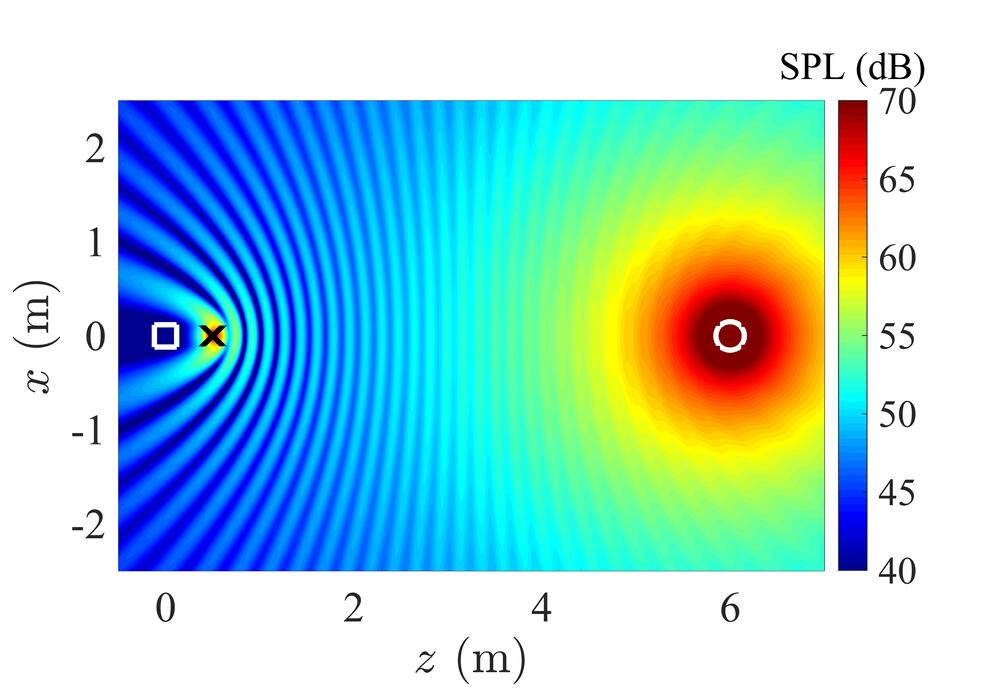
\includegraphics[width = 1\textwidth]{fig/cal_ANC_demo_On_1kHz_SecPointMonopole_dse0p5m_resize.jpg}
        \caption{}
    \end{subfigure}
    \begin{subfigure}{0.49\textwidth}
        \centering
        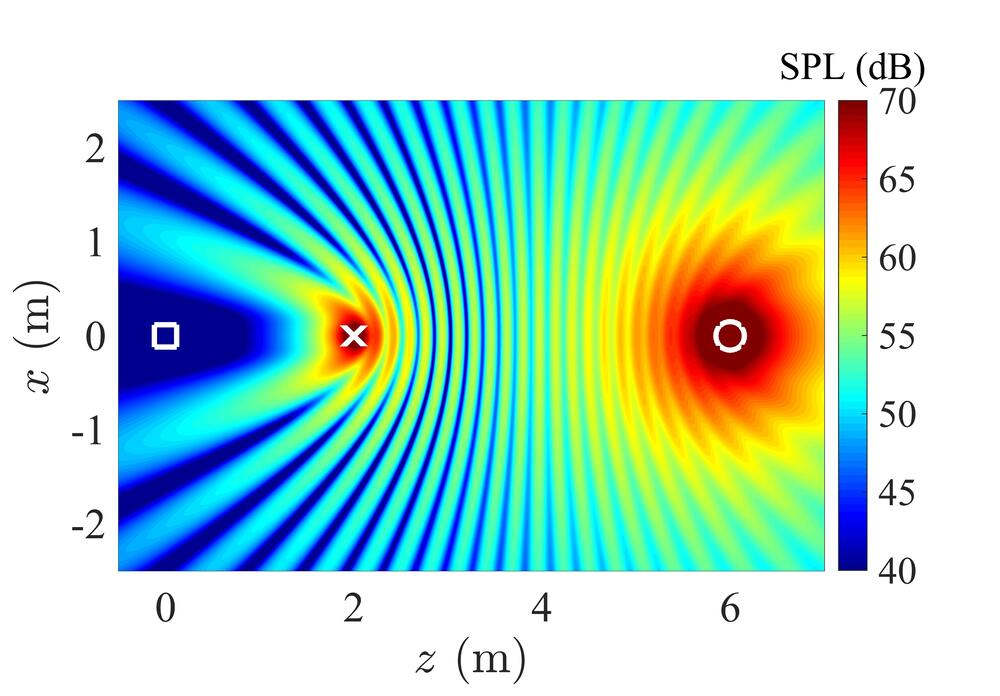
\includegraphics[width = 1\textwidth]{fig/cal_ANC_demo_On_1kHz_SecPointMonopole_dse2m_resize.jpg}
        \caption{}
    \end{subfigure}
    \caption{\revA{SPL (dB re 20 $\mu$Pa)} generated by a point source located at $(x,z) = (0,\SI{6}{m})$ at 1 kHz and the sound at the $(x,z) = (0,0)$ is controlled by a traditional omnidirectional loudspeaker at: (a) $(x,z) = (0, \SI{0.5}{m})$; and (b) $(x,z) = (0,\SI{2}{m})$. Circle, primary source; cross, secondary source; square, error point.}
    \label{fig:anc_change_dist}
\end{figure}

% The single channel ANC system shown in Figs. \ref{fig:intro:389fsdp} and \ref{fig:anc_change_dist} can creat only one
% If multiple quiet zones or a larger quiet zone 
    The spillover effect is also occurred in the  multi-channel local active control system, which aims to create multiple quiet zones or a larger quiet zone using multiple secondary sources \cite{Nelson1992ActiveControlSound}. 
    For example for a binaural ANC system as shown in Fig.~\ref{fig:intro:tanaka2017model}, two secondary sources are introduced to mitigate the noise at two ears.
    The secondary field at each ear is the superposition of the sound waves radiated by two secondary loudspeakers.
    Except for two secondary paths between either loudspeakers and the ipsilateral ears, there are another two crosstalk secondary paths between either loudspeakers and the contralateral ears.
    If the secondary source is omnidirectional, the crosstalk secondary paths are non-negligible and must be taken into account in signal processing algorithms. 
    They would double the computational cost in the ANC controller \cite{Tanaka2017BinauralActiveNoise}.

\begin{figure}[!htb]
    \centering
    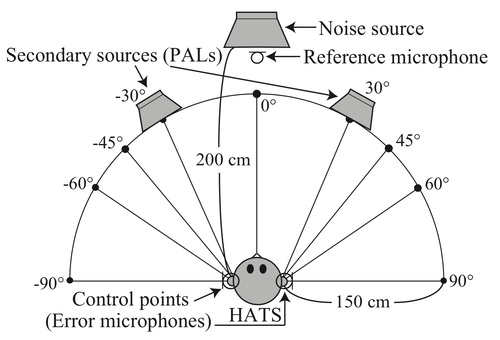
\includegraphics[width = 0.5\textwidth]{Figures/pending/Tanaka2017-Model_resize.jpg}
    \caption{Sketch of a binaural ANC system using two PALs. From Fig. 6 in \cite{Tanaka2017BinauralActiveNoise}.}
    \label{fig:intro:tanaka2017model}
\end{figure}


% Some studies have demonstrated the capabilities and potentials of using directional sources to eliminate the spillover effect \cite{Mangiante1977ActiveSoundAbsorption, Chen2011ActiveNoiseBarrier, Hu2019ActiveCancellationSound}. 
The sound waves radiated by directional sources focus on their propagation axis, and have small effects in other directions.
Owing to this feature, using directional sources in ANC systems can mitigate the spillover effect \cite{Mangiante1977ActiveSoundAbsorption, Chen2011ActiveNoiseBarrier, Hu2019ActiveCancellationSound} as well as reduce the crosstalk secondary paths \cite{Tanaka2014MultichannelActiveNoise, Tanaka2017BinauralActiveNoise}. 
Parametric array loudspeakers (PALs) are a special kind of loudspeakers, which has sharp radiation directivity when compared to existing traditional dynamic loudspeakers. %, and is therefore a promising secondary source for ANC systems. 
The sharp directivity for PALs can be clearly identified in a comparison of the sound field radiated by a PAL and a traditional loudspeaker of the same radiation surface, as shown in  Fig.~\ref{fig:pal_sound_field_compare_to_traditional}.
The advantage of using PALs in ANC systems has been demonstrated in some studies \cite{Tanaka2010ActiveNoiseControl, Tanaka2011MathematicallyTrivialControl, Tanaka2014MultichannelActiveNoise, Tanaka2017BinauralActiveNoise}. 
For example, after replacing the omnidirectional secondary source in Fig.~\ref{fig:anc_change_dist} by the PAL, the noise reduction performance is shown in Fig.~\ref{fig:anc_change_dist_pal} and , it is clear the spillover effect is much reduced.
However, most existing studies focus on using one or two PALs to cancel the noise at error points, where the generated quiet zone is rather small.
It is necessary to investigate the feasibility of using multiple PALs to generate a large quiet zone.

\begin{figure}[!htb]
    \centering
    \begin{subfigure}{0.47\textwidth}
        \centering
        % \includegraphics[width=\textwidth]{E:/UTS/CandidatureAssessment/CA1/slides/img/show_2D_audio1000_PistonSource_A_resize.jpg}
        \includegraphics[width=\textwidth]{fig/show_2D_audio1000_PistonSource_A_resize.jpg}
        \caption{}
    \end{subfigure}
    \begin{subfigure}{0.47\textwidth}
        \centering
        % \includegraphics[width=\textwidth]{E:/UTS/CandidatureAssessment/CA1/slides/img/show_2D_audio1000_ultra60e3_A_resize.jpg}
        \includegraphics[width=\textwidth]{fig/show_2D_audio1000_ultra60e3_A_resize.jpg}
        \caption{}
    \end{subfigure}
    \caption{\revA{SPL (dB re 20 $\mu$Pa)} at 1 kHz generated by: (a) a traditional loudspeaker; (b) a PAL located at the origin and of the same radiation surface.}
    \label{fig:pal_sound_field_compare_to_traditional}
\end{figure}

\begin{figure}[!htb]
    \centering
    \begin{subfigure}{0.49\textwidth}
        \centering
        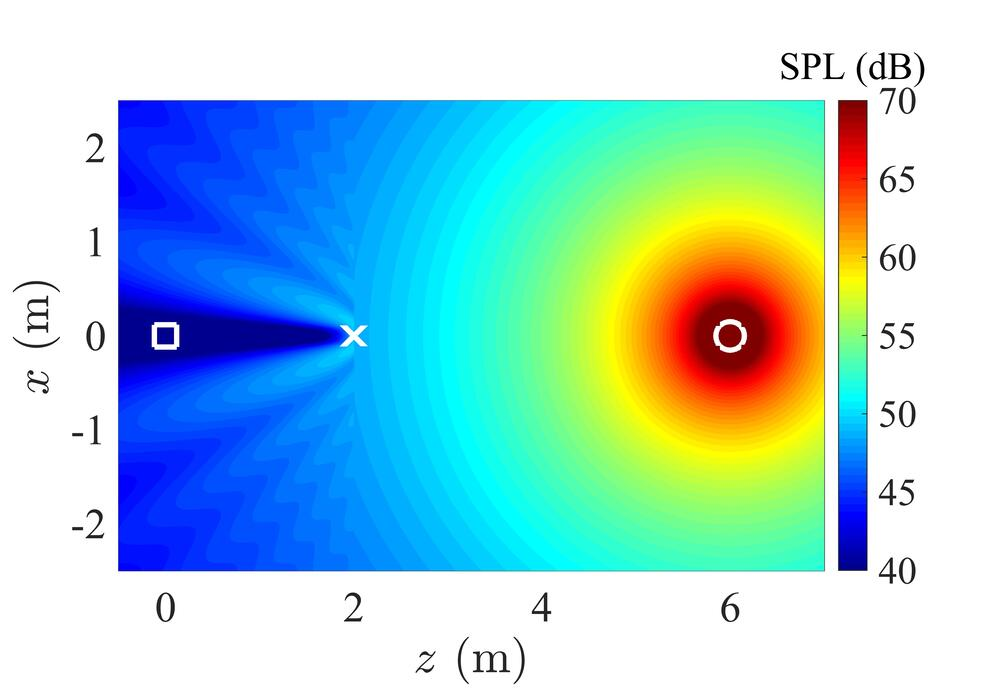
\includegraphics[width = 1\textwidth]{fig/cal_ANC_demo_On_1kHz_SecPAL_dse2m_resize.jpg}
        \caption{}
    \end{subfigure}
    \begin{subfigure}{0.49\textwidth}
        \centering
        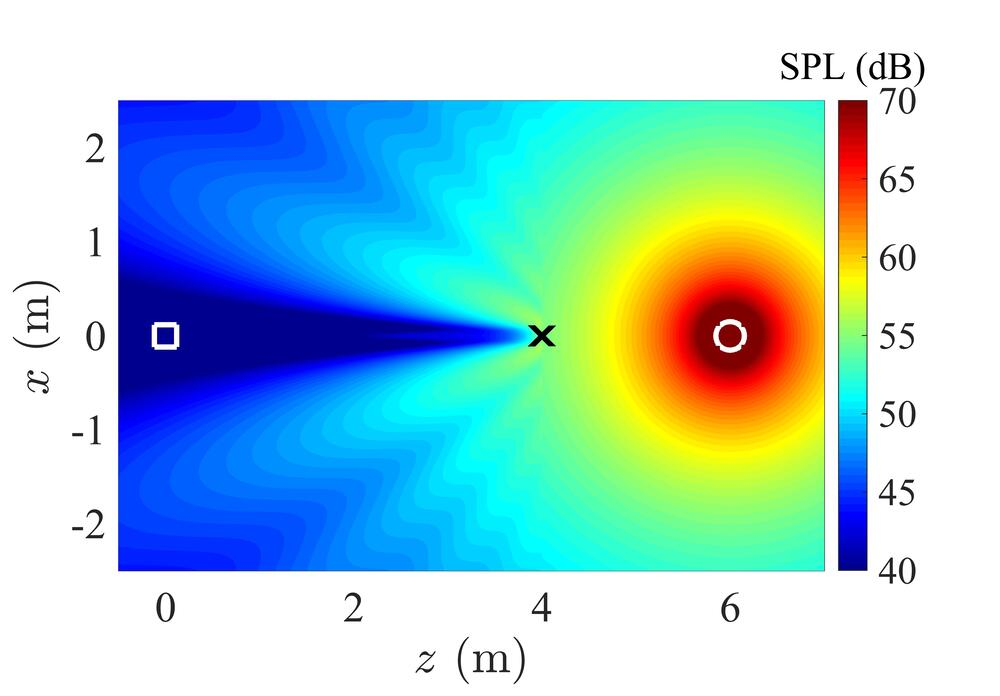
\includegraphics[width = 1\textwidth]{fig/cal_ANC_demo_On_1kHz_SecPAL_dse4m_resize.jpg}
        \caption{}
    \end{subfigure}
    \caption{
        \revA{SPL (dB re 20 $\mu$Pa)} generated by a point source located at $(x,z) = (0,\SI{6}{m})$ at 1 kHz and the sound at the $(x,z) = (0,0)$ is controlled by a PAL at: (a) $(x,z) = (0, \SI{0.5}{m})$; and (b) $(x,z) = (0,\SI{2}{m})$. 
    \revA{Circle, primary source; cross, secondary source; square, error point.}}
    \label{fig:anc_change_dist_pal}
\end{figure}

    ANC and related audio systems are used in various kinds of acoustic environments, where the sound waves experience the reflection, transmission, scattering, and other physical phenomena. 
    % These properties have significant effects on the noise reduction performance of ANC systems.
    When traditional dynamic loudspeakers are adopted as secondary sources, they are usually modelled as point monopoles at low frequencies, the theory of which is trivial. 
    At middle and high frequencies, more accurate models can be used to predict the sound field, such as the model taking into account the radiation directivity or the aperture size of the loudspeakers.
    The theory for traditional dynamic loudspeakers has been well developed and used in investigating the effects of the physical properties of secondary sources on ANC performance.
    For example, it has been demonstrated that the noise reduction performance can be much improved by optimally setting the locations of secondary sources and reflecting surfaces for both global and local active control \cite{Boodoo2015ReviewEffectReflective, Tao2017PerformanceMultichannelActive, Zhong2019IncreasingPerformanceActive, Zhong2019IncreasingPerformanceActivea, Zhong2020PerformanceActiveNoise};
    the ANC system can be used to increase the insertion loss of a passive partition \cite{Sas1995ActiveControlSound, Tarabini2009ActiveControlNoisea, Zhang2017PerformanceSnoringNoise} and enclosures \cite{Dupont2009ActiveAbsorptionReduce};
    the scattering effects caused by a human head is beneficial to the ANC system in terms of performance robustness with regard to the movements of the human head \cite{Lin2004ActiveControlRadiation, Zou2008PerformanceAnalysisVirtual, Liu2018ActiveControlStrategy, Elliott2020ActiveControlSound}.
    All of aforementioned studies demonstrate the physical properties (e.g., reflection, transmission, and scattering) of secondary sources have significant effects on the performance of ANC systems.
    % However, The generation of audio sound by a PAL is a nonlinear process, and the theory is more complicated than the traditional loudspeakers.
    However, these properties for audio sound generated by PALs are still unclear, which will be investigated in this thesis.
    % The active partition (a passive partition integrated with an ANC system) can increase the insertion loss of the partition

% For the applications in the field of ANC, it is necessary to know the physical properties of the sound waves generated by secondary sources in various kinds of acoustic environments, such as the reflection from a reflecting surface \cite{Boodoo2015ReviewEffectReflective, Tao2017PerformanceMultichannelActive, Zhong2019IncreasingPerformanceActive, Zhong2019IncreasingPerformanceActivea, Zhong2020PerformanceActiveNoise}, transmission through a partition \cite{Sas1995ActiveControlSound, Tarabini2009ActiveControlNoisea, Zhang2017PerformanceSnoringNoise}, and scattering by a human head \cite{Lin2004ActiveControlRadiation, Zou2008PerformanceAnalysisVirtual, Liu2018ActiveControlStrategy, Elliott2020ActiveControlSound}. 
% Although the theoretical research on predication models for the audio sound generated by a PAL has continued to date (e.g., \cite{Shi2012ProductDirectivityModels, Shi2015ConvolutionModelComputing, Cervenka2013NonparaxialModelParametric, Guasch2018FarfieldDirectivityParametric, Cervenka2019VersatileComputationalApproach} for details), there are still a lot to do to improve the calculation efficiency and accuracy for PALs in different acoustic environments. 

\section{Objectives}
% This thesis focuses on the investigation of prediction models, physical properties of audio sound generated by a PAL, and the applications in ANC systems as secondary sources to create a large quiet zone.
% The objectives of this thesis lie in the following three aspects in the field of PAL and ANC.
The primary aim of this thesis is to investigate the feasibility of using multiple PALs in an ANC system to create a large quiet zone.
This thesis aims to improve the fundamental understanding of how PALs affect the noise reduction performance and the quiet zone size in a multi-channel ANC systems.
In particular, since heavy computations for the audio sound generated by PALs are required in modelling the noise reduction performance of a multi-channel ANC system, a new partial-wave expansion method is proposed to reduce the computational load without causing loss of accuracy. 
In addition, the proposed method is extended to investigate the reflection, transmission, and scattering phenomena for PALs, which are common in real applications but the relevant studies are rare.
Finally, the proposed model incorporated with the multi-channel ANC theory is used to investigate the quiet zone size controlled by multiple PALs.
The spillover effect will be evaluated quantitatively and compared to the systems using traditional dynamic loudspeakers which have omnidirectional radiation pattern.

% \noindent\paragraph{Objective 1}\mbox{}\\

% The accurate calculation of audio sound generated by a PAL is rather time-consuming due to the evaluations of five-fold integrals \cite{Cervenka2019VersatileComputationalApproach}. 
% The existing method employs the paraxial (Fresnel) approximation to simplify the calculations which is inaccurate at wide angles from the radiation axis of the PAL \cite{Cervenka2013NonparaxialModelParametric}. 
% Therefore, it is worth investigating whether it is possible to simplify the calculation without additional approximations. 
% The existing method is based on a baffled model; however, it has been reported that audio sound can be heard behind a PAL in free field (non-baffled model). 
% It is necessarily to develop a theoretical model which can predict the sound on both front and back sides of a non-baffled PAL.

% \noindent\paragraph{Objective 2}\mbox{}\\

% The audio sound generated by PALs can be treated as the superposition of the sound generated by infinitely many virtual sources in space with the source density proportional to the product of the sound pressure of ultrasound. 
% Therefore, the formation of the audio sound is accumulated before the ultrasound being totally absorbed in air. 
% There would be interesting phenomena if the accumulation process is truncated by a reflecting surface, blocked by a partition, or scattered by a sphere (simulating a human head).
% The results and conclusions are also useful for applications of PALs in ANC systems.

% \noindent\paragraph{Objective 3}\mbox{}\\

% It has been reported that PALs can be used in ANC systems to create a quiet zone around the target point without affecting the sound levels in the other areas. 
% However, the existing studies focus only on the control of the pure tone or  narrow band (upper limit is less than 2.5 kHz) noise \cite{Tanaka2010ActiveNoiseControl, Tanaka2014MultichannelActiveNoise, Tanaka2011MathematicallyTrivialControl, Tanaka2017BinauralActiveNoise}.
% The feasibility of applying PALs to reduce broader band noise up to 6 kHz remains to be investigated, as well as the feasibility of creating a large quiet zone with multiple PALs.


\section{Thesis outline}
The structure of the thesis is as follows:

\noindent\paragraph{Chapter \ref{chap:intro}: \nameref{chap:intro}}\mbox{}\\

This chapter gives a brief introduction on the concepts of PAL and ANC, and the motivation and objectives of this thesis.
The thesis outline and contributions are also presented.

\noindent\paragraph{Chapter \ref{chap:review}: \nameref{chap:review}}\mbox{}\\

This chapter presents a systematic review of PAL and ANC.
For PALs, it includes the physical mechanism and properties of the audio sound generated by a PAL, 
the prediction models, implementations and applications. 
For ANC, it includes the methods to generate a quiet zone and ANC systems using directional loudspeakers and PALs.

\noindent\paragraph{Chapter \ref{chap:sound_field}: \nameref{chap:sound_field}}\mbox{}\\

This chapter firstly reviews the governing equations for audio sound generated by a PAL.
The quasilinear solutions for both three-dimensional and two-dimensional models are presented.
The front side for a baffled PAL is proposed to be divided into three regions: the near field, the Westervelt far field, and the inverse-law far field.
The widely used \revA{Gaussian beam expansion (GBE)} model and the convolution model are concluded to predict the sound fields in the Westervelt far field and the inverse-law far field, respectively.
The sound field on the back side for a non-baffled PAL is predicted using the non-paraxial PAL model and the disk scattering theory.
Experimental results are presented to validate the proposed model.

\noindent\paragraph{Chapter \ref{chap:predict_model}: \nameref{chap:predict_model}}\mbox{}\\

This chapter proposes two improved prediction models for PALs.
The first model is called the \revA{spherical wave expansion (SWE)} model which is used to calculate the radiation from a circular piston source, and the audio sound generated by a circular PAL.
The second model is called the \revA{cylindrical wave expansion (CWE)} model which is used to calculate the audio sound generated by a phased array PAL.
The advantages of the proposed models are illustrated by numerical simulations.

\noindent\paragraph{Chapter \ref{chap:phys}: \nameref{chap:phys}} \mbox{}\\

This chapter provides a systematic investigation on the physical properties for audio sound generated by a PAL.
The reflection of audio sound generated by a PAL is investigated first when an infinitely large reflecting surface is placed near the PAL. 
A theoretical model is then developed to predict the transmission of audio sound generated by a PAL through a thin partition, and is used to quantitatively analyze the insertion loss. 
The scattering effects of a rigid sphere (simulating a human head) on audio sound generated by a PAL are investigated.
Experimental results are presented to validate the models proposed in this chapter.

\noindent\paragraph{Chapter \ref{chap:anc}: \nameref{chap:anc}} \mbox{}\\

This chapter investigates the feasibility of using a PAL to reduce a broadband (up to 6 kHz) noise at the human ears.
Then the feasibility of using multiple PALs to create a large quiet zone is investigated, and the physical limitations are explored. 
Experiments of both single and  multi-channel ANC systems are conducted to verify the findings.

\noindent\paragraph{Chapter \ref{chap:conclusion}: \nameref{chap:conclusion}} \mbox{}\\

This chapter concludes the work in this chapter.
The future work and outlook are also presented. 

\section{Contributions}
The main original contributions of this thesis are as follows:
\begin{outline}[enumerate]
    \1 A spherical wave expansion method for calculating the audio sound generated by a PAL has been proposed for both Westervelt \cite{Zhong2020SphericalExpansionAudio} and Kuznetsov \cite{Zhong2021FieldWesterveltFar} equations.
    The proposed method is found to be not only more accurate but also 15 times faster than the widely used Gaussian beam expansion method, and is more than 100 times faster than the direct integration method without any loss of accuracy.
    \1 A closed-form solution for calculating the radiation from a circular piston source has been proposed using the spherical wave expansion method \cite{Zhong2020SphericalExpansionCalculating}.
    \1 A cylindrical wave expansion method for calculating the audio sound generated by a phased array PAL has been proposed \cite{Zhong2021CylindricalExpansionAudio}.
    It improves the agreement with the experimental results when compared to the existing convolution model.
    \1 The reflection from a reflecting surface \cite{Zhong2020ReflectionAudioSounds}, the transmission through a thin partition \cite{Zhong2020InsertionLossThin}, and the scattering by a rigid sphere (simulating a human head) \cite{Zhong2022ScatteringRigidSphere}, for audio sound generated by a PAL have been investigated by both simulations and experiments.
    The work provides a framework and a guidance for investigating these physical properties of audio sound generated by a PAL.
    \1 An ANC system has been designed and implemented to cancel the noise at human ears, where the secondary source is a commercial PAL and the error signal is remotely detected by an optical microphone using the laser Doppler vibrometer technique \cite{Zhong2020ExperimentalStudyActive}.
    Experiments are conducted to test the performance of such a system.
    \1 The feasibility of using multiple PALs to create a large quiet zone has been validated by both simulations and experiments \cite{Zhong2022QuietZoneGeneration}.
    The empirical formulae to estimate the quiet zone size have been proposed.
\end{outline}

